\documentclass{scrartcl}[12pt, halfparskip]
\usepackage[utf8x]{inputenc}
\usepackage[T1]{fontenc}
\usepackage[english]{babel}
\usepackage{amsmath, amssymb, amstext}
\usepackage{wrapfig}
\usepackage{float}
\usepackage{graphicx}
\usepackage{color}
\usepackage{algorithm}
\usepackage[noend]{algpseudocode}

\usepackage{caption}
\usepackage{subcaption}


\setlength{\parindent}{0pt}

\newcommand{\todo}[1]{\textcolor{red}{TODO: #1}}


\title{Seminar Combinatorial Optimization}
\author{Jan Lammel}
\date{\today{}, Heidelberg}



\begin{document}

\maketitle \ \\ 
\newpage


\section{Introduction}
In this work there will be presented the results of Yuri Boykov et al. \cite{boykov98}, \cite{boykov01} to solve computer vision problems like image segmentation. First we will explain the mathematical framework, including the relation to the segmentation vision problem we want to solve. Afterwards two approximative algorithms are introduced in order to solve the problem efficiently. Finally we will show some outcomes of this method on real data.


\section{Mathematics}
In computer vision tasks we handle with images containing pixels $P = \{ 1, 2, ..., m \}$. Each of these pixels have two attributes in terms of random variables, observation $O$ and hypothesis $f$. In the task of image segmentation the observation $O$ would be for example the result of normalized correlation (see ...) and $f \in \mathcal{L}^m$ with $\mathcal{L} = \{l_1,l_ 2, ..., l_k\}$ are the k labels of the segmentation pattern we are finally looking for (see ...). \\


\subsection{Maximum a posteriori (MAP) estimate}

So in the end we want $f$ s.t. $p(f|O)$ is maximized, called $f^*$. Using Bayes' rule

\begin{equation}
	p(f|O) \propto p(O|f) p(f)
\end{equation}

means that we need expressions for $p(O|f)$ and $p(f)$.


\subsection{Markov Random Fields (MRFs)}
The system of pixels (including their random variables $f_p$ and $O_p$) can be drawn as a graph where each pixel is represented by a node. In a Markov Random Field all neighboring pixels are connected with an edge (see ...). 

Due to the Hammersley-Clifford theorem, which states that the prior term can be written as sum of potentials in an exponential functions, it holds for our MRF:
\begin{equation}
	p(f) \propto \exp\{ - \sum\limits_{p \in \mathcal{P}} \sum\limits_{q \in \mathcal{N}_p} V_{pq} (f_p, f_q) \}
\end{equation}
where $\mathcal{N}_p$ are the neighboring pixels of $p$ and $V_{pq}$ is the potential between pixel $p$ and $q$. This term is usually used to smooth the solution, i.e. penalize different neighboring labels $f_p \neq f_q$.

Examples for potentials $V_{pq}$ are
\begin{itemize}
	\item Generalized Potts model: $V_{pq}(f_p, f_q) = u_{pq} (1 - \delta(f_p - f_q))$
	\item Truncated quadratic distance: $V_{pq}(f_p, f_q) = \min (K=const, |f_p - f_q|^2)$
	\item Truncated $L_2$ norm: $V_{pq}(f_p, f_q) = ???$
\end{itemize}

The other term $p(O|f)$ is often called data term because here we are using the information of the input image we want to segment. For this term we are using the independend and identical distributed (iid) assumption so we get

\begin{equation}
	p(O|f) = \prod\limits_{p \in \mathcal{P}} g(i, p, f_p)
\end{equation}

where $g \in [0, 1]$. Examples ??? \\
\todo{mit $D_p(\alpha)$ schreiben wie in 2. Paper...} \\

Due to the fact that we want to maximize $p(f)$ we can take the negative logarithm (which is monotonic and therefore doesnt change the position of the extremum) and minimize the resultung Energy function

\begin{equation}
E(f) = - \ln(p(f)) = \sum\limits_{p \in \mathcal{P}} \sum\limits_{q \in \mathcal{N}_p} V_{pq} (f_p, f_q) - \sum\limits_{p \in \mathcal{P}} \ln(g(i, p, f_p))
\end{equation}
\label{eq:energy-function}

In general for $k$ labels and $m$ pixels there are $k^m$ possible states of $f$. A common image contains for example $m = 800 \times 600 = 480,000$ pixels, means even for just $k = 2$ labels in the case of a foreground-background segmentation there are $k^m \approx 10^{144,000}$ possible configurations for $f$. This is a lot more than the number of (fermion) particles in our universe.

Because of this it would be useful being able to reduce the number of possible states:

In general if $E(f^*)$ is finite, one can always find some constant $K(p)$ for each pixel $p$ s.t. the following holds:

\begin{equation}
	- \ln(g(i, p, f_p^*)) < K(p)
\end{equation}

It will be further explained by taking $K(p) = E(f)$, which one always use if no better argument is available. Given some $E(f)$ we can drop all labels $l$ of pixel $p$ where $- \ln(g(i, p, l)) > E(f)$ because this data term alone is higher than the energy we found. The other terms will just increase it even more. So we can define label sets for each pixel
\begin{equation}
	\mathcal{L}_p = \{l \in \mathcal{L}: \ - \ln(g(i, p, l)) < E(f) \}
\end{equation}
with labels which are able to decrease the energy value in comparison to the one we already found $E(f)$.

\todo{Abgeaenderte Energy function mit h statt g... wobei ich nicht kapier warum die aequivalenz gilt...}


\subsection{Multiway Cut Problem}
In order to solve this combinatorial optimization problem efficiently we build up a new graph $\mathcal{G} = \langle \mathcal{V} = \mathcal{V}_p \cup \mathcal{V}_t, \mathcal{E} = \mathcal{E}_n \cup \mathcal{E}_n \rangle$ the following way:

In total there are $m$ nodes $\mathcal{V}_p$ for each pixel and $k$ so called terminal nodes $\mathcal{V}_t$ for all labels. Now there are two kinds of edges. First so called t-links $\mathcal{E}_t$ between each pixel and the terminals according to the reduced label sets $\mathcal{L}_p$. Each t-link is assigned the weight
\begin{equation}
	V_{p,l} = h(i,p,l) + \sum\limits_{q \in \mathcal{N}_p} V_{p,q}
\end{equation}
\todo{Verstehe nicht wirklich warum hier noch n-links drin sind...}

On the other hand n-links $\mathcal{E}_n$ between neighbouring pixels with the weight

\begin{equation}
	V_{p,q} = 2 u_{p,q}
\end{equation}

\todo{Formel gilt nur fuer Potts-model... was wenn z.b. truncated squared model?}

\textbf{Definition: \textit{multiway cut}}\\
A multiway cut is a subset $\mathcal{C} \subset \mathcal{E}$ of the graph's edges such that all terminals are no longer connected via edges in the induced graph $\mathcal{G}(\mathcal{C}) = \langle \mathcal{V}, \mathcal{E} - \mathcal{C}\rangle$. The cost of the cut $|\mathcal{C}|$ is the sum over all cutted edge's weights. 

The minimum multiway cut problem is to find the multiway cut which minimizes $|\mathcal{C}|$. \\

\textbf{Definition: \textit{feasability multiway cut}}\\
A multiway cut is called feasible if each pixel node is left connected with exactly one terminal node in $\mathcal{G}(\mathcal{C})$. \\


It can be proven that a minimum cost multiway cut $\mathcal{C}$ on $\mathcal{G}$ for terminals $\mathcal{L}$ must be feasible \cite{boykov98} and furthermore if $\mathcal{C}$ is a minimum cost multiway cut on $\mathcal{G}$, then the corresponding labeling $f^C$ minimizes $E(f)$ in \eqref{eq:energy-function} \cite{boykov98}.





\section{Approximative Algorithms for the Multiway Cut Problem}
Due to the fact that solving the whole multiway cut problem exactly is NP-complete we are forced to use approximative methods in order to solve the problem in a reasonable time.
The following algorithms are based on comparing just two different labels at once, that is a usual min-cut problem which can be solved in near-linear time.


\subsection{$\alpha$-$\beta$ swap}

\todo{Weights?!}

\begin{wrapfigure}{r}{0.5\textwidth} 
	\vspace{-1.5cm}
	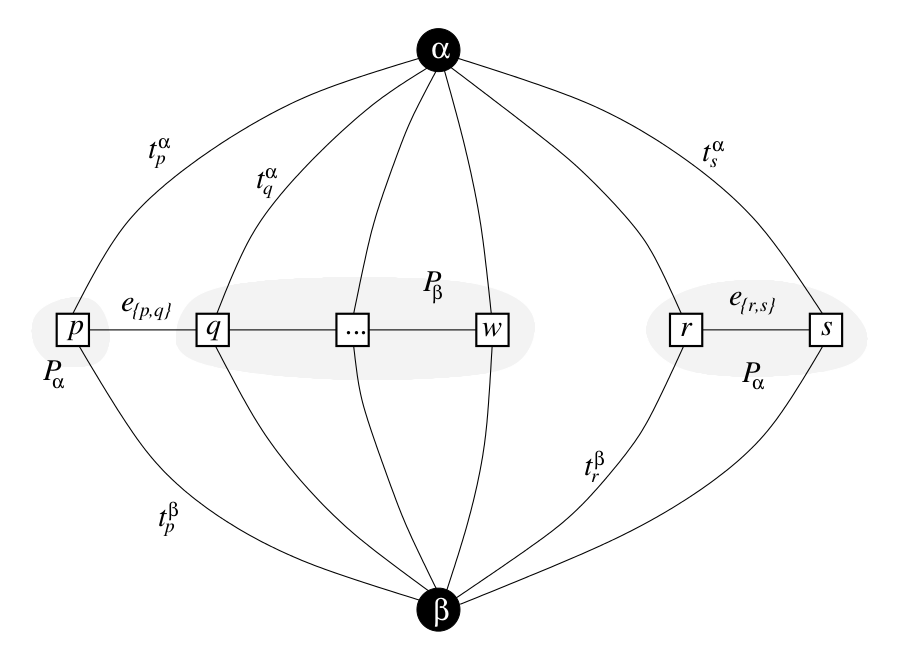
\includegraphics[width=0.5\textwidth]{/home/argo/seminar/data/alpha-beta-swap_Gab.png}
	\caption{blubb}
	\label{fig:alpha-beta-swap_Gab}
\end{wrapfigure}

The first algorithm $\alpha$-$\beta$ swap is shown in Algorithm \ref{alg:alpha-beta-swap}. In each iteration in step 6 we just consider the subgraph $\mathcal{G}_{\alpha \beta} = \langle \mathcal{V}_{\alpha \beta}, \mathcal{E}_{\alpha \beta} \rangle$, i.e. just take the pixels into account which have been labeled $\alpha$ or $\beta$ before (see Fig. \ref{fig:alpha-beta-swap_Gab}) and find the corresponding minimum cut. This is done for all possible pairs of labels. If some swap achieve a lower energy $E(\hat{f})$ of the complete graph $\mathcal{G}$, the labeling will be updated. If no possible swap improve the result further, the algorithm has finished. \\

Within the subproblem of finding the minimum cut of $\mathcal{G}_{\alpha \beta}$ cutting the terminal $t_p^\alpha$ assigns pixel $p$ label $\alpha$. 
All pixels $p \notin \mathcal{P}_{\alpha \beta}$ keep obviously the same label as before. 


The different case of cuts are shown in Figure \ref{fig:alpha-beta-swap_Gab_cuts}.


\begin{figure}[H]
	\begin{subfigure}{0.32\textwidth}
		\centering
		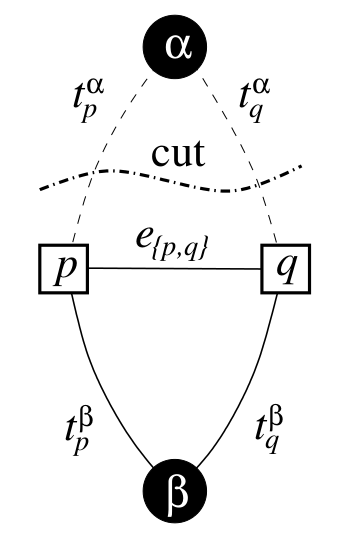
\includegraphics[width=1.0\textwidth]{/home/argo/seminar/data/alpha-beta-swap_Gab_cut1.png}
		\caption{}
		\label{fig:alpha-beta-swap_Gab_cut1}
	\end{subfigure}
	\begin{subfigure}{0.32\textwidth}
		\centering
		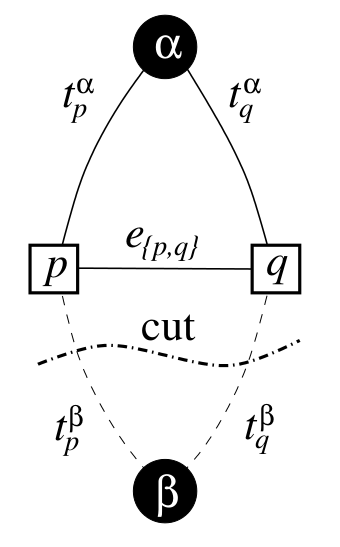
\includegraphics[width=1.0\textwidth]{/home/argo/seminar/data/alpha-beta-swap_Gab_cut2.png}
		\caption{}
		\label{fig:alpha-beta-swap_Gab_cut2}
	\end{subfigure}
	\begin{subfigure}{0.32\textwidth}
		\centering
		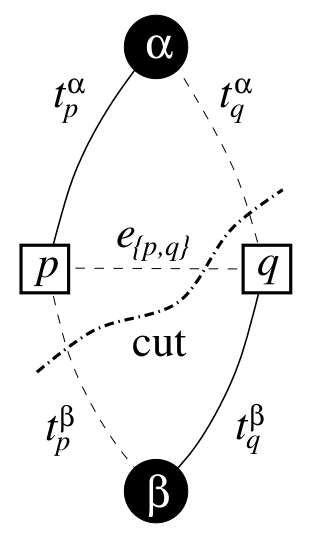
\includegraphics[width=1.0\textwidth]{/home/argo/seminar/data/alpha-beta-swap_Gab_cut3.png}
		\caption{}
		\label{fig:alpha-beta-swap_Gab_cut3}
	\end{subfigure}
\caption{}
\label{fig:alpha-beta-swap_Gab_cuts}
\end{figure}


Choosing the edge weights properly conducts to the following main results: \\

\textbf{Theorem:}\\
There is a one to one correspondence between cuts $\mathcal{C}$ on $\mathcal{G}_{\alpha \beta}$ and labelings that are one $\alpha$-$\beta$ swap away from $f$. Moreover, the cost of a cut $\mathcal{C}$ on $\mathcal{G}_{\alpha \beta}$ is $|\mathcal{C}| = E(f^\mathcal{C})$ plus a constant. \\

\textbf{Corollary:}\\
The optimal $\alpha$-$\beta$ swap from $f$ is $\hat{f} = f^\mathcal{C}$ where $\mathcal{C}$ is the minimum cut on $\mathcal{G}_{\alpha \beta}$. \\


I.e. the labeling $\hat{f}$, which we get in step 6 of Algorithm \ref{alg:alpha-beta-swap} is a local minimum in the sense of switching some labels $\alpha$ and $\beta$ won't decrease the energy function's value of the whole graph $\mathcal{G}$. Further this means when the algorithm has terminated, any swap with two arbitrary labels won't achieve a lower energy which is a local minima in an extended move space.



\begin{algorithm}[H]
\caption{$\alpha$-$\beta$ swap}\label{alg:alpha-beta-swap}
\begin{algorithmic}[1]
\Procedure{AlphaBetaSwap($f$)}{}
	\State $f$: (Arbitrary) initial labeling 
	\State
	\State Set $success = 0$
	\For{each pair of labels $\{\alpha, \beta\} \subset \mathcal{L}$ }:
		\State Find $\hat{f} = \arg \min E(f')$ among $f'$ within one $\alpha-\beta$ swap of $f$
		\If{$E(\hat{f}) < E(f)$}:
			\State Set $f := \hat{f}$
			\State Set $success = 1$
		\EndIf
	\EndFor
	\If{$success == 1$}:
		\State go to step 4
	\EndIf
	\State
	\State \Return{$f$}
\EndProcedure
\end{algorithmic}
\end{algorithm}








\subsection{$\alpha$-expansion}



\begin{figure}[H]
	\begin{subfigure}{0.32\textwidth}
		\centering
		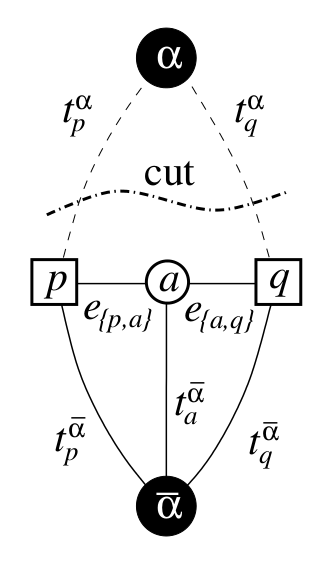
\includegraphics[width=1.0\textwidth]{/home/argo/seminar/data/alpha-expansion_cut1.png}
		\caption{}
		\label{fig:alpha-expansion_Gab_cut1}
	\end{subfigure}
	\begin{subfigure}{0.32\textwidth}
		\centering
		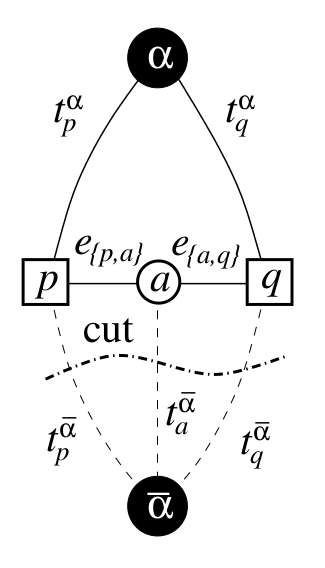
\includegraphics[width=1.0\textwidth]{/home/argo/seminar/data/alpha-expansion_cut2.png}
		\caption{}
		\label{fig:alpha-expansion_Gab_cut2}
	\end{subfigure}
	\begin{subfigure}{0.32\textwidth}
		\centering
		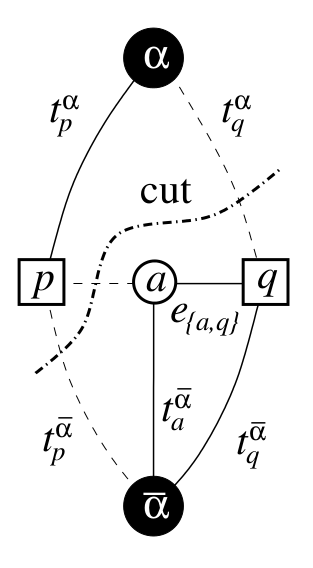
\includegraphics[width=1.0\textwidth]{/home/argo/seminar/data/alpha-expansion_cut3.png}
		\caption{}
		\label{fig:alpha-expansion_Gab_cut3}
	\end{subfigure}
\label{fig:alpha-expansion_Gab_cuts}
\caption{}
\end{figure}



\begin{algorithm}[H]
\caption{$\alpha$-expansion}\label{alg:alpha-expansion}
\begin{algorithmic}[1]
\Procedure{AlphaExpansion($f$)}{}
	\State $f$: (Arbitrary) initial labeling 
	\State
	\State Set $success = 0$
	\For{each label $\alpha \in \mathcal{L}$ }:
		\State Find $\hat{f} = \arg \min E(f')$ among $f'$ within one $\alpha$-expansion of $f$
		\If{$E(\hat{f}) < E(f)$}:
			\State Set $f := \hat{f}$
			\State Set $success = 1$
		\EndIf
	\EndFor
	\If{$success == 1$}:
		\State go to step 4
	\EndIf
	\State
	\State \Return{$f$}
\EndProcedure
\end{algorithmic}
\end{algorithm}


\section{Applications in Vision problems}
\subsection{Image restoration}
\subsection{Segmentation}




\begin{thebibliography}{9}

\bibitem{boykov98}
  Yuri Boykov, Olga Veksler and Ramin Zabih:
  Markov Random Fields with Efficient Approximations,
  1998,
  IEEE Computer Society Conference on Computer Vision and
  Pattern Recognition
  
\bibitem{boykov01}
  Yuri Boykov, Olga Veksler and Ramin Zabih:
  Fast Approximate Energy Minimization via Graph
  Cuts,
  IEEE Transactions on Pattern Analysis and Machine Intelligence archive Volume,
  23 Issue 11, November 2001 Page 1222-1239
  

  

\end{thebibliography}

\end{document}